
\documentclass{article}

%\usepackage{amsmath}
%\usepackage{apacite}
%\usepackage[pdftex]{graphicx}
\usepackage{graphicx}
\usepackage{mslapa}
\usepackage[section]{placeins}  % place a \FloatBarrier in each section
\usepackage{url}
\usepackage{fullpage}  % to standard 1 inch margins

\raggedright

\begin{document}
\setlength{\parindent}{1cm}

\title{Engine Tuning with Msqdev}
\author{Jeremiah Mahler}
\date{\today}

\maketitle

\tableofcontents

\pagebreak

\section{Introduction}

The Megasquirt \cite{MEGA11} engine controller allows for the
control of nearly every possible parameter of a running engine.
But this wide spectrum of parameters also makes it difficult to tune.
The typical tuning method \cite{MEGAMAN} is based on rules of thumb
and imprecise judgements of performance.
The Msqdev system \cite{MAHL11} was created to provide a
methodical method of tuning with provable metrics of performance.

The design of Msqdev consists of various parts.
In general small robust programs are preferred over large all encompassing ones.
The \verb+msqdev+ daemon creates the interface to the ecu.
It monitors a directory of files which describe the settings and
communicates over the serial port to the Megasquirt ecu when these
files are changed or need to be updated.
There are utilities such as \verb+msq-ve_tuner+ for automatically
tuning the fuel mixture and \verb+msq-accel_tuner+ for performing
acceleration tuning as well as many others.
The utilities are small since they only read and write files and it
is easy to create new ones.
Plotting and analysis of captured data is most often done using
R \cite{R} scripts.

\subsection{Installation}

This project is still in early development and the installation
described here allows for updates to be easily performed.

The first step is to retrieve a copy of the current project.
The best way is by using Git \cite{GIT} with the command below.
If Git is not not available the package can be downloaded and unpacked
directly.
The recommended placement is in the users directory (\verb+~/msqdev+)
which is the default if the git clone command is run in the home directory.

\begin{verbatim}
git clone https://github.com/jmahler/msqdev.git
\end{verbatim}

After the Msqdev package has been successfully retrieved and unpacked
it is necessary to compile the \verb+msqdev+ daemon.
This is done by changing to the \verb+msqdev/src/+ directory and typing
\verb+make+.
If all goes correctly the \verb+msqdev+ executable will be produced.

In order to access the binaries from any location it is necessary to
configure the users \verb+PATH+.
The recommended way is to add the \verb+~/bin+ to the \verb+PATH+ environment
variable and then to create symbolic links from inside \verb+bin+ directory
to those in \verb+msqdev+.

\begin{verbatim}
jeri@bishop ~$ ls ~/bin | grep msq
msq-accel_tuner
msq-afr_table
msqdev
msq-point_values
msq-rtmonitor
msq-speed_tuner
msq-table_points
msq-ve_tuner
jeri@bishop ~$ grep PATH ~/.bashrc
export PATH="$HOME/bin:$PATH"
jeri@bishop ~$ env | grep PATH
PATH=/home/jeri/bin:/usr/local/bin:/usr/bin:/bin
ri/QuizMaker/bin:/home/jeri/QuizMaker/bin
\end{verbatim}

The final step is to verify that \verb+msqdev+ works.
The following is an example of the steps used on one system.

\begin{verbatim}
jeri@bishop ~$ mkdir tmp-msqdev
jeri@bishop ~$ cd tmp-msqdev
jeri@bishop tmp-msqdev$ ls  # directory is empty
jeri@bishop tmp-msqdev$ msqdev /dev/ttyUSB0 
Mon Jul  4 16:34:17 2011: start
Mon Jul  4 16:34:31 2011: updating files from ecu
^Cjeri@bishop tmp-msqdev$   # quit by Ctrl-C
jeri@bishop tmp-msqdev$ ls  # msqdev created files
advanceTable1  afrTable1  pid  rtdata  veTable1
\end{verbatim}

\section{Steady State Tuning}
\label{sec:steadytun}

Steady state tuning is done when the engine rpms are stable such as
at idle.
Its use under heavier load conditions is possible but it is difficult to
balance load exactly to the power output.

Steady state tuning is performed by altering variables and then measuring
the new steady state.
As an example consider varying the fuel mixture at idle to maximize rpm.
In a range around the current mixture each setting has a corresponding
rpm (see Figure \ref{fig:sstrpm}).
The setting closest to the maximum is the best setting.

% TODO - rebuild this as a pdf so it looks better
\begin{figure}[tbp]
\center
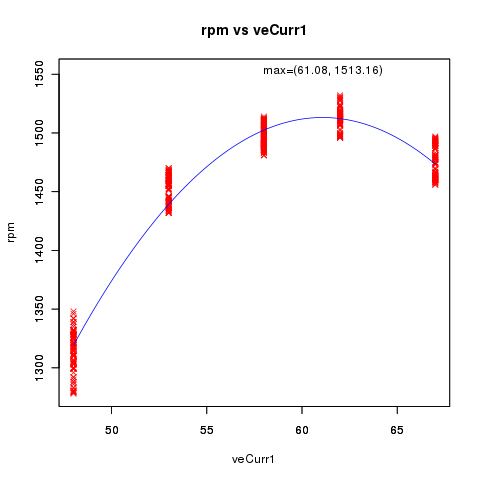
\includegraphics[scale=0.5]{plot01}
\caption{Steady State Tuning by varying veCurr1 vs rpm at idle.}
\label{fig:sstrpm}
\end{figure}

The order in which the variables are varied can be helpful in detecting
if there is any error caused by acceleration.
Suppose, for example that the engine rpms were decelerating.
If the variables were varied from one boundary to the other it would have
decreasing slope.
If instead the variables were varied from the center to one boundary and then
back to the center to the other boundary the center point will be
separated if there was any acceleration (Figure \ref{fig:ssrerr}).

% TODO - rebuild this as a pdf so it looks better
\begin{figure}[tbp]
\center
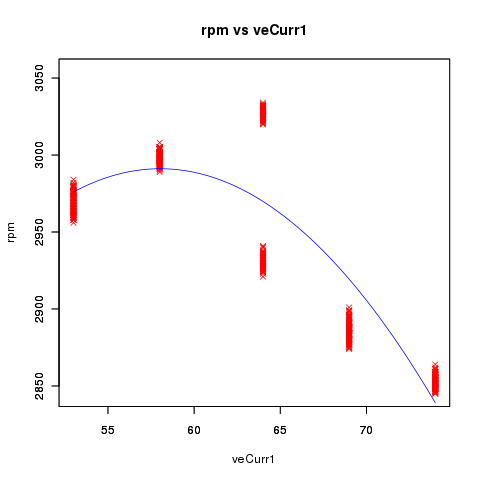
\includegraphics[scale=0.5]{plotdata-veTable1-20110613-15:17:10.png}
\caption{Steady state tuning with a large deceleration error
indicated by the gap in the center..}
\label{fig:ssrerr}
\end{figure}

\subsection{convergence of VE tuning}

It would be useful to know whether the changes that are being made
converge to some stable value.
Suppose the goal is to achieve some air fuel ratio and we are in a
limited range of the ve map, such as at idle.
The changes of each of these points can be plotted over time and
if they stabilizing they will reach a constant value.

To display this data it needs to be arranged in a certain way.
In this example we will be using R\cite{R} and Ggplot2\cite{wickham2009ggplot2}.

The data file should consist of the following values:
\begin{itemize}
\item time - Time in seconds.
\item veCurr1 - The current ve setting.
\item group - A unique identifier for a point such as X-Y, where
  X and Y are the unique row and column.
\end{itemize}

\section{Acceleration Tuning}
\label{sec:acctun}

In contrast to Steady State Tuning (Section \ref{sec:steadytun}), Acceleration
Tuning is done when the engine rpms are increasing or decreasing.
This method is more useful than Steady State Tuning because it can be
applied to far more situations and does not depend on balanced conditions.

One source of error with acceleration tuning is with the throttle position.
A human operator is quite imprecise and can easily allow significant
throttle movement without their knowledge.
To reduce this error a throttle stop can be used.
The throttle stop is a fixed length object such as a piece of tubing which
can be placed underneath the gas pedal to limit its travel.
Support in the tuning program can provided to start/stop recording so
that a trial is only recording while the pedal is against the stop.

\begin{figure}[!htbp]
\center
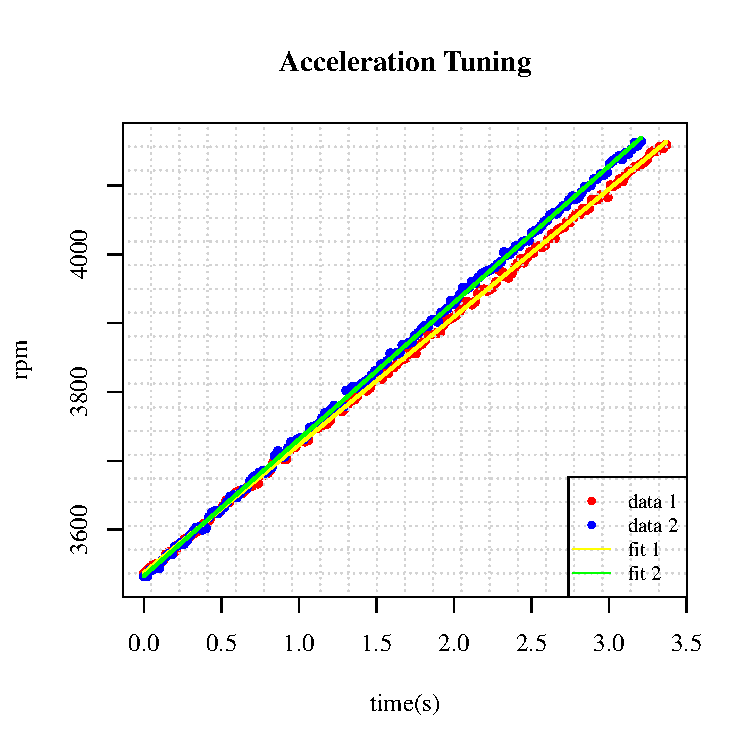
\includegraphics[scale=0.8]{msq-accel-4g_52cm_45-65mph-20110627-20:17:43-rtdata-single}
\caption{Comparison of two acceleration tuning trials.
Each trial is constrained to the same range of rpms.
Because the second trial reached the given rpm in a shorter time
period it maximized acceleration compared to the first trial.}
\label{fig:acctun}
\end{figure}

As can be seen from Figure \ref{fig:acctun} Acceleration Tuning is good
at discerning differences over a range which result in a cummulative
difference.
It would be very poor a discerening a few marginal adjustments.
The values should be varied by considering this characteristic.
When adjusting the ve table, for example, multiple values over the
range should adjusted.
If the adjustments could be made to produce a constant air fuel ratio
over a trial this could be beneficial in finding the ratio that produces
the greatest acceleration.
Predicting air fuel ratios will be discussed in Section \ref{sec:predafr}.

\section{Air Fuel Ratio}
\label{sec:afr}

% good introduction
The fuel mixture is crucial in determining how well an engine runs.
If it is too rich or too lean the engine will lack power.
To minimize emissions the stoichiometric mixture is best.
To maximize power a richer than stoichiometric mixture is best.
To maximize fuel economy a leaner than stoichiometric mixture is best.
Obviously only one of these can be maximized at a time for a given
point on the map.
In general the goal of any of these is to achieve a specific fuel
mixture for specific operating conditions.

The desired air fuel ratio can be found by incrementally adjusting
values while the engine is running until the desired value is achieved.
This procedure also results in many data samples of settings and their
resulting air fuel ratios.
To go beyond merely achieving a single desired air fuel ratio, this data
can be used to build a function which predicts what the air
fuel ratio will be.
This has the added benefit of being able to instantly set the air fuel ratio
to any desired value.

\subsection{Predicting Air Fuel Ratios}
\label{sec:predafr}

% procedure, step 1
The first step in building a function which can predict the air fuel ratio
is to record data.
This is accomplished in the Msqdev system using \verb+msq-ve_tuner+ utility.
This utility will attempt to adjust the current ve values to achieve
a specific air fuel ratio.
The engine should be run through various rpm ranges and various load values.
Whether the desired air fuel ratio is achieved is not important,
rather data samples of the air fuel ratio for a given setting are what
matter.

% procedure, step 2
Once an adequate data sample has been recorded it can be processed 
using the R script \verb+afr_predict.R+ (Appendix \ref{app:afrpred})
which performs a least squares fit to find the coefficients which define
the linear function.
These coefficients can then be used with the Msqdev utility \verb+msq-afr_table+
to build tables with any desired air fuel ratio.



There are several sources of error when predicting air fuel ratios.
Acceleration enrichment would skew the results because additional
fuel is added which is not accounted for.
This error can be eliminated by disabling enrichment or by only
moving the throttle slowly.
Another source of error is with the delay between when settings are
executed and when the oxygen sensor reads the value.
Wide band Oxygen sensor response times are typically very fast it
is estimated that the delay would be no more the a half second.
More work is needed to determine the magnitude of these errors and
how they can be compensated for.

\FloatBarrier  % keep all the figures in this section

\subsection{Finding The Air Fuel Ratio For Maximum Power}
\label{sec:findafrpow}

Once the function which predicts the air fuel ratio has been found
(Section \ref{sec:predafr}) the values can be varied to find which
one produces the maximum power (maximum acceleration).
In the Msqdev system this is accomplished using the utility
\verb+msq-accel_tuner+ for performing acceleration tuning (Section \ref{sec:acctun}).

A good general starting point for tuning the air fuel ratio is to
configure the table so that a constant air fuel ratio is produced
during a trial.
Then the air fuel ratio can be adjusted during subsequent trials and
their performance compared.

\appendix
\section{afr\_predict.R}
\label{app:afrpred}

% The following text was generated by appA-ve_tuner.tex.php
% Thu, 19 Jan 2012 12:43:23 -0800

\begin{verbatim}

# This script is used to perform a least squares fit of the data
# related to veTable1 to find the function that predicts the
# air fuel ratio.

# To run this script start R and source this file
#
# bash$ R
# > source("afr_predict.R")
# Loading required package: MASS
# 
# Call: rlm(formula = afr1 ~ veCurr1 + fuelload + rpm, maxit = 40)
# Residuals:
#     Min      1Q  Median      3Q     Max 
# -4.1269 -0.4980 -0.1448  0.5697  3.0852 
# 
# Coefficients:
#             Value    Std. Error t value 
# (Intercept)  17.9873   0.0925   194.3936
# veCurr1      -0.1399   0.0023   -61.2773
# fuelload      0.0525   0.0016    33.8201
# rpm           0.0004   0.0000    25.2164
# 
# Residual standard error: 0.7837 on 12986 degrees of freedom
# >

# Once the coefficients are found a table can be built using
# the command below (with different values).
#
# bash$ msq-afr_table -afr 16.5 -a -0.1399 -b 0.0525 -c 0.0004 -d 17.9873

# Choose the file with the recorded data from msq-ve_tuner
#f1 <- "20110626-ve_tuner/msq-ve_tuner-20110626-16:47:48" # ok
f1 <- "20110626-ve_tuner/msq-ve_tuner-20110626-16:59:22" # good
#f1 <- "20110626-ve_tuner/msq-ve_tuner-20110626-17:12:36"  # ok

d1 <- read.csv(file=f1, head=TRUE, sep=",")


# Filter the data to remove invalid extreme values.

# Remove invalid extreme air fuel ratios
filt0 <- d1$afr1 > 10 & d1$afr1 < 16

# remove invalid idle and deceleration values
filt0 <- filt0 & d1$tps > 1

# remove near idle rpms
filt0 <- filt0 & d1$rpm > 2600

veCurr1  <- d1$veCurr1[filt0]  	# x
afr1 	 <- d1$afr1[filt0]  	# y
fuelload <- d1$fuelload[filt0]  # z
rpm 	 <- d1$rpm[filt0]


# account for delay in afr1
# TODO - how does the filtering (above) affect the delay?  Is it correct?
dX <- 0  # ok
#dX <- 10  # ok
#dX <- 20  # ok
#dX <- 40
#dX <- 60  # too far
# shift forward
afr1 <- afr1[(dX + 1):length(afr1)]
# shift back
veCurr1 <- veCurr1[1:(length(veCurr1) - dX)]
fuelload <- fuelload[1:(length(fuelload) - dX)]
rpm <- rpm[1:(length(rpm) - dX)]

#lmfit1 <- lm(formula = afr1 ~ veCurr1 + fuelload + rpm)
require(MASS)  # rlm
lmfit1 <- rlm(formula = afr1 ~ veCurr1 + fuelload + rpm, maxit=40)

print(summary(lmfit1))

\end{verbatim}


\pagebreak

\bibliographystyle{mslapa}
%\bibliographystyle{plain}
%\bibliographystyle{acm}
%\bibliographystyle{ieeetr}
\bibliography{main}

\end{document}
